\begin{frame}{Support Vector Classifiers (SVC)}

\begin{itemize}
    \item In \textbf{SVC} we consider a hyperplane that does not perfectly separate the two classes, in the interest of: \pause 

    \begin{itemize}
        \item[\checkmark] Greater robustness to individual observations. \pause 

        \item[\checkmark] Better classification of most of the training observations. \pause 
    \end{itemize}

    \item We do not seek the largest possible margin so that \textbf{every observation} is classified perfectly. \pause 
    
    \item We allow some observations to be on the incorrect side of the margin, or even the incorrect side of the hyperplane. \pause 
\end{itemize}

\begin{figure}
    \centering
    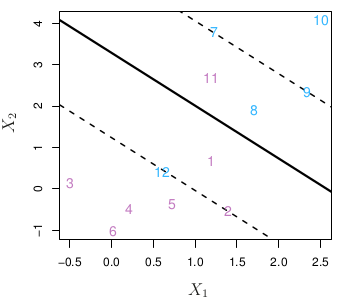
\includegraphics[height=4cm]{svc/soft-margin.png}
\end{figure}
    
\end{frame}